\documentclass[10pt,oneside]{article}
\usepackage{amsmath} % Símbolos refinados de matemáticas
\usepackage{graphicx} % Incluir imágenes
\usepackage{subcaption} % Poder usar subfiguras
\usepackage{amsfonts}
\usepackage{amssymb} % Los símbolos el los conjuntos numéricos
\usepackage{subfig}

% Opciones de lenguaje usando polyglossia (defino dos para este documento)
\usepackage{polyglossia}
\setmainlanguage{spanish}
\setotherlanguage[variant=american]{english}


% El sistema de bibliógrafa es Biber (no necesitas BibTeX)
\usepackage[
  backend=biber
]{biblatex}
\addbibresource{biblio.bib}

% Márgenes y tamaño del papel
\usepackage[
  letterpaper,
  left=2cm,
  right=2cm,
  top=1.5cm,
  bottom=1.5cm
]{geometry}

% Poner los links en azul y definir los meta-datos del pdf
\usepackage[
  final,
  unicode,
  colorlinks=true,
  citecolor=blue,
  linkcolor=blue,
  plainpages=false,
  urlcolor=blue,
  pdfpagelabels=true,
  pdfsubject={Métodos Climatológicos},
  pdfauthor={Matías Briceño},
  pdftitle={Tarea 1},
  pdfkeywords={}
]{hyperref}

% Tablas con estilo profesional
\usepackage{booktabs}

% Para poner algoritmos en pseudo código
\usepackage{algpseudocode}
\usepackage{algorithm} %Ambiente flotante para los algoritmos
%Hacer los comentarios en el pseudocódigo como en C++
%\algrenewcommand{\algorithmiccomment}[1]{\hskip3em$//$ #1}
\floatname{algorithm}{Algoritmo}

% Definición del encabezado y del pies de página
\usepackage{lastpage}
\usepackage{fancyhdr}
\fancyhf{}
\pagestyle{fancy}
\fancyhf{}
\fancyhead[L]{Universidad de Chile - Departamento de Geofísica} %Nombre de la materia
\fancyhead[C]{} % Nombre del alumno
\fancyhead[R]{\href{https://github.com/Mabriceno/MC_T4}{https://github.com/Mabriceno/MC_T4}} % Repositorio
\fancyfoot[R]{Profesores: Sergio González - Juan P. Boisier}
% https://tex.stackexchange.com/questions/227/how-can-i-add-page-of-on-my-document
\fancyfoot[C]{\thepage\ of \pageref*{LastPage}}
%\fancyfoot[C]{ of }
\fancyfoot[L]{Métodos Climatológicos} % Grupo
\renewcommand{\headrulewidth}{2pt} 
\renewcommand{\footrulewidth}{2pt}

\usepackage[newfloat=true]{minted} %Para insertar código fuente en algún lenguaje de programación
% Requiere que compiles usando:
% $xelatex -shell-escape input.tex

% Para el correcto funcionamiento, esta plantilla debe compilarse así:
% 1 XeLaTeX
% 2 Biber 
%    Antes de 20.04 esta herramienta no estaba en los repositorios oficiales de Ubuntu
%    ver: https://tex.stackexchange.com/questions/154751/biblatex-with-biber-configuring-my-editor-to-avoid-undefined-citations/154763#154763)
% 3 XeLaTex
% 4 XeLateX
% 5 ViewPDF

\author{Matías Briceño} %Como el nombre del autor ya viene en el encabezado
\title{Tarea 4}
% Si por alguna razón la fecha que deseas que aparezca no es la de hoy
% \usepackage{datetime}
% \newdate{date}{06}{09}{2012}
% \date{\displaydate{date}}
\date{9 de junio de 2022}

% Configuración del entorno minted para poner código fuente
\DeclareCaptionFormat{mitedFormat}{%
    \textbf{#1#2}#3}
\DeclareCaptionStyle{minetdStyle}{skip=0cm,width=.85\textwidth,justification=centering,
  font=footnotesize,singlelinecheck=off,format=mitedFormat,labelsep=space}
\newenvironment{mintedCode}{\captionsetup{type=listing,style=minetdStyle}}{}

\usepackage{dirtytalk} % Para usar comillas

% Cambia el nombre de la etiqueta. Afecta a todos los códigos minted del documento
\SetupFloatingEnvironment{listing}{name=Código}
% Opciones de minted para el lenguaje C++
\setminted[cpp]{frame=lines,framesep=0.25cm,baselinestretch=1,fontsize=\scriptsize,breaklines}
% Cuando lo hagas dentro de un párrafo el tamaño de fuente debe ser normal
\setmintedinline[cpp]{fontsize=auto}

\setlength{\parindent}{2 pt} % Quita las sangrías

\usepackage{csquotes} % Por que si no esta presente AQUI polyglossia tira un warning

\begin{document}

\maketitle
\thispagestyle{fancy} %Para que los fancy headers estén desde la primera página
% El cuerpo de la tarea esta en este otro archivo



\section*{Parte 1. Análisis armónico para ciclo estacional}

\bigskip

Para este análisis se utilizaron registros diarios de precipitación y caudal de la cuenca del río de Trancura en la región de la Araucanía. Se consideró el periodo 1979-2018. Se realizaron tratamientos previos al análisis en cada uno de los sets de datos que consistieron en la eliminación de días bisiestos para un correcto análsis armónico y el reemplazo de días faltantes por el valor medio de la serie.  

\bigskip

A través de un análisis de Fourier se calcularon los tres armónicos principales con los cuales suele representarse ciclos estacionales (T = 365 días, T/2 y  T/3). En cada uno de los casos el cálculo se hizo con una regresión lineal multiple para conseguir las amplitudes respectivas. Además, se calcularon las medias para cada uno de los días de tal manera de encontrar el ciclo estacional medio. Los resultados se pueden ver en la \textbf{Figura 1}.  

\bigskip

El cilo estacional de precipitación muestra un pick esperable en el período de invierno que se puede apreciar en las dos técnicas utilizadas. La media muestra gran ruido, que está relacionado con la naturaleza de la distribución de esta variable dado que las precipitaciones cercanas a cero son más probables. El ciclo estacional del caudal presenta dos picks importantes, el primero y con mayor amplitud ocurre durante el mismo período que el pick del ciclo de precipitación que podría implicar una correlación entre ambas variables. El segundo pick podría estar relacionado a otros fenómenos como la temperatura, dado que ocurre en un período en el que típicamente las temperaturas comienzan a subir. Una explicación podría ser el deshielo. 

\begin{figure}[htp]
\centering
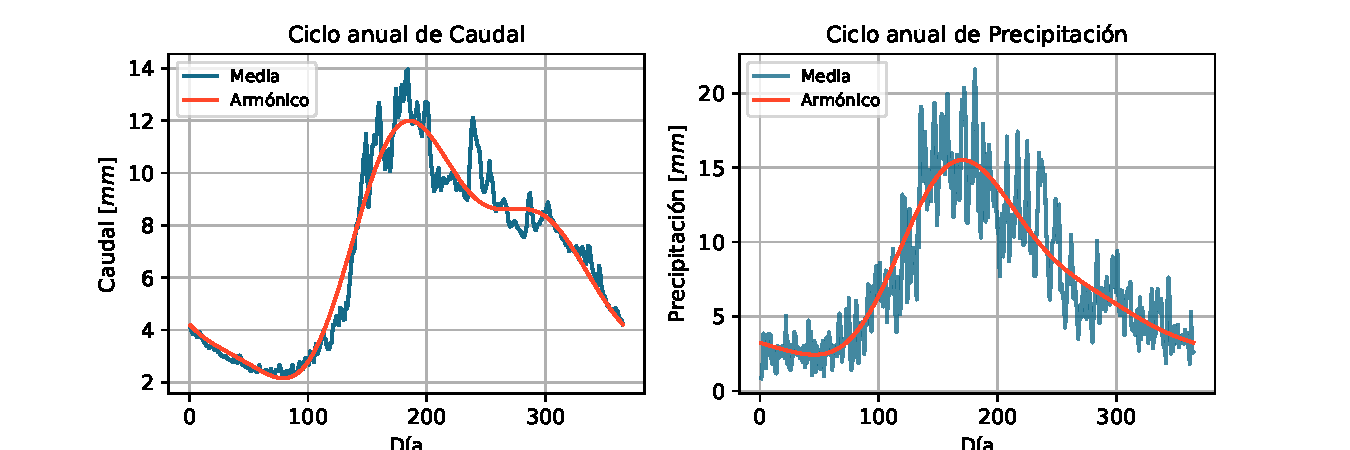
\includegraphics[width=1\textwidth]{img/ciclos.pdf}
\caption{\textbf{Ciclos estacionarios de Caudal y Precipitación, Cuenca Trancura.} Los ciclos fueron calculados a partir de 40 años de muestra (1979-2018). }
\label{fig:1}
\end{figure}

\newpage

\section*{Parte 2. Análisis espectral de anomalías}

\bigskip

Para esta sección se hizo un análisis armónico sobre las anomalías históricas de las mismas series trabajadas previamente. Para el cálculo de las anomalías se utilizó la diferencia entre el ciclo estacional dado por los tres armónicos principales y los registros curados. Se utilizó la Trasformada de Fourier Rápida (\textit{fft}) dado que el cómputo necesario para utilizar el método de regresión lineal es importante. La \textbf{Figura 2} muestra los periodogramas para cada espectro calculado. Se observa que el poder espectral en ambos espectros tienen un patrón similar.

\bigskip


\begin{figure}[htp!]
\centering
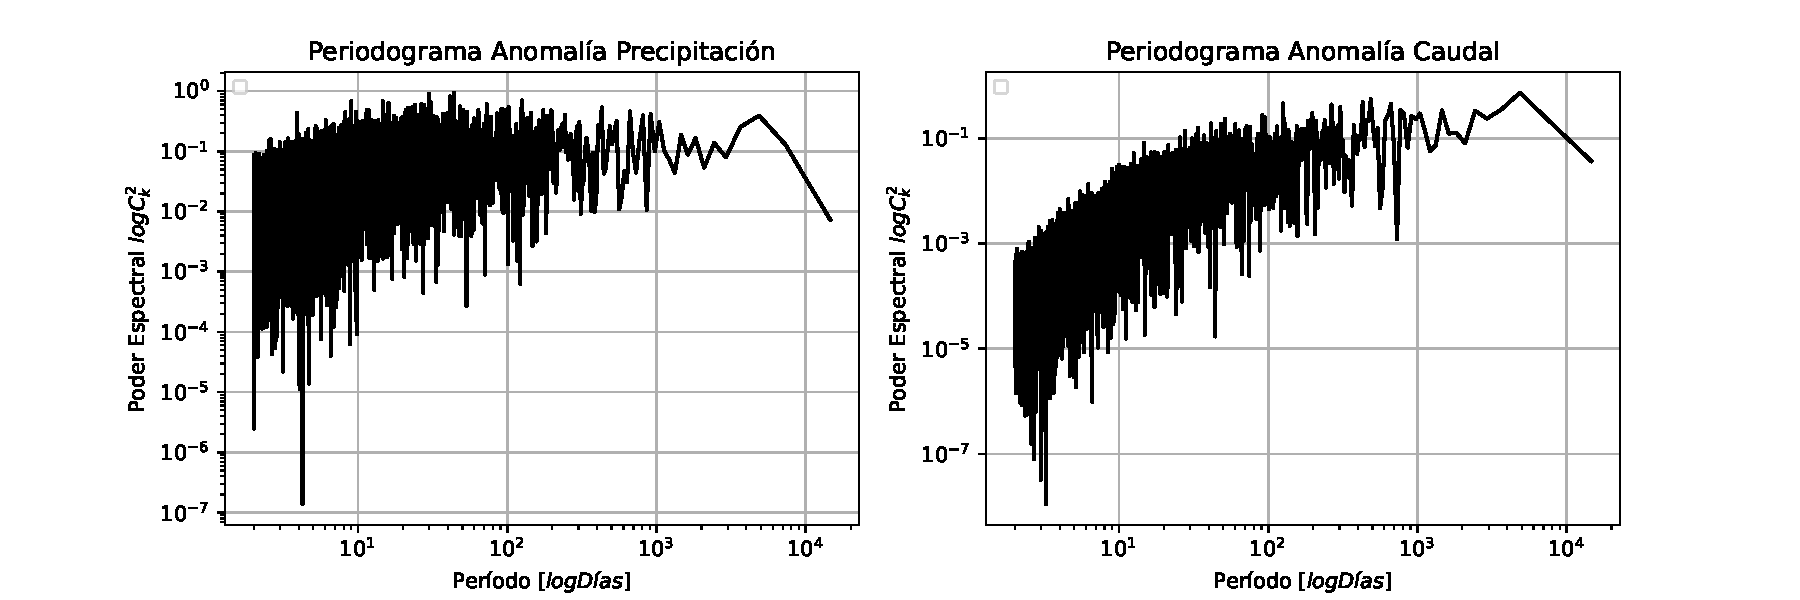
\includegraphics[width=1\textwidth]{img/spectral.pdf} 
\caption{\textbf{Periodogramas de anomalías diarias de Caudal y Precipitación.} Se presenta el poder espectral para cada período utilizado.}
\label{fig:5}
\end{figure}
\bigskip

\newpage

\bigskip

\section*{Parte 3. Modelos lineales para prediccíon de Anomalía del Caudal}

\bigskip

De la misma manera que en la primera parte de este informe, se calcularon los ciclos estacionales para conseguir las series de anomalías de caudal y precipitación, pero esta vez de los registros mensuales con el objetivo de construir un modelo que sea capaz explicar la variación de las anomalías del caudal a partir de las anomalías de precipitación. El primer modelo (\textit{modelo 1}) consistió en una regresión lineal simple entre ambas series. Los resultados de este modelo asi como las series anomalas se pueden ver en la \textbf{Figura 3}. El $R_{2}$ entre la serie de Anomalía del caudal y las predicciones del \textit{modelo 1} fue de $0.48$.

\bigskip

\begin{figure}[htp!]
\centering
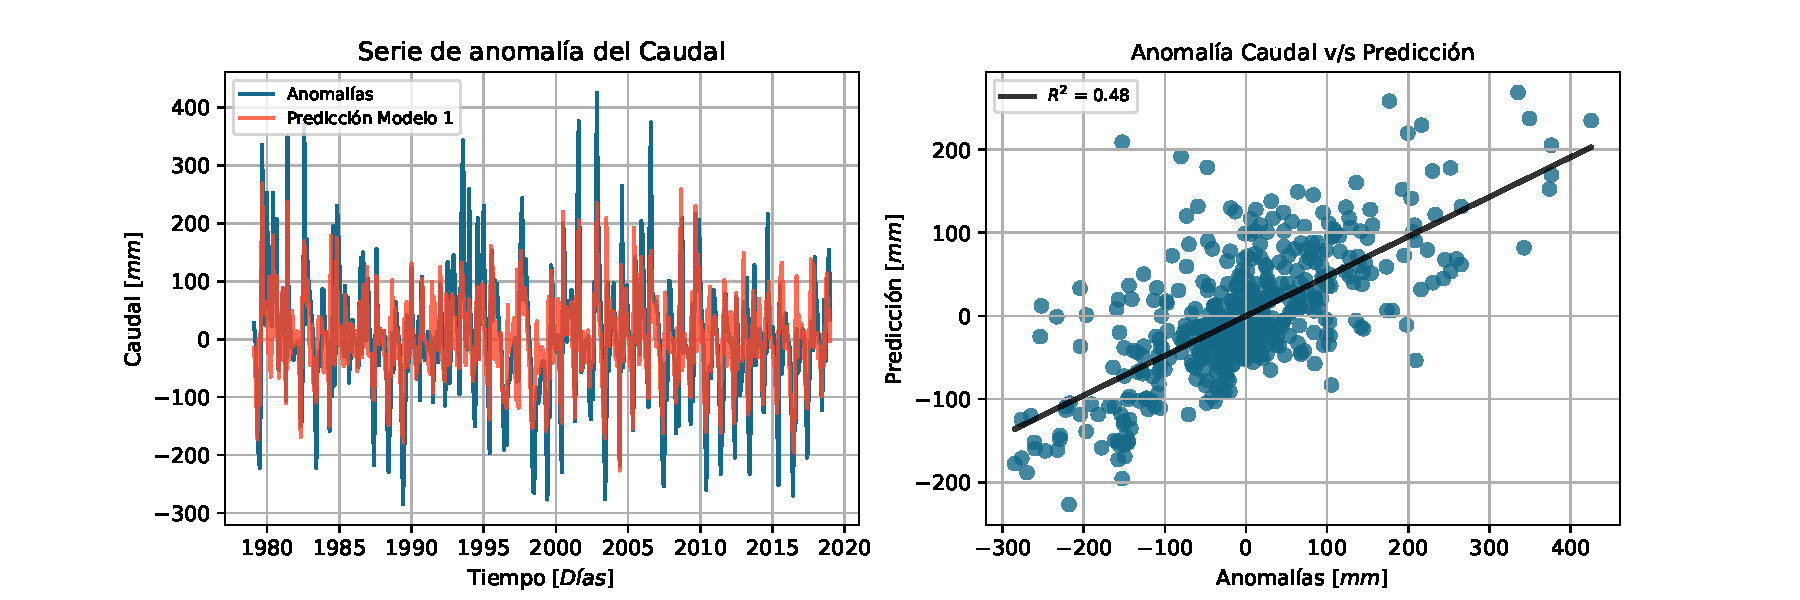
\includegraphics[width=1\textwidth]{img/model1.pdf}
\caption{\textbf{Modelo 1 para anomalías de caudal, Cuenca Trancura.} La figura izquierda muestra la serie de anomalías del caudal junto con la estimada con el \textit{modelo 1}. La figura derecha muestra un diagrama de dispersión entre ambas series.}
\label{fig:8}
\end{figure}

\bigskip

Se construyeron otros tres modelos multivariados usando desfases de 1, 2 y 3 meses. El \textit{modelo 2} agrega un desfase de 1 mes, el \textit{modelo 3}agrea desfases de 1 y 2 meses y el \textit{modelo 3} agrega desfases de 1, 2 y 3 meses. Los resultados muestran que al agregar variables al modelo este aumenta en 0.02  el $R^{2}$ entre la variables inicial y su prediccón por lo que las nuevas variables no están aportando información demasiado relevante para explicar la variabilidad de la anomalía, quizás, por un problema de multicolinealidad (correlación entre las mismas variables de entrada). Una opción sería agregar mas variables para complejizar el modelo, pero esto podría llevar a un problema de sobreajuste que no sería bueno si se quiere utilizar el modelo para hacer predicciones con datos que no se utilizaron en el entrenamiento.  

\bigskip

Para evaluar este patrón y en qué punto el modelo se sobre ajusta se iteró la técnica anterior 300 veces agregando cada vez mas variables de desfase. Los analisis se pueden ver en la \textbf{Figura 4}. Es interesante notar que el crecimiento del $R^{2}$ no es acelerado sino que casi constante, habiendo puntos en los que no crece (multicolinealidad). Antes de llegar a las 250 iteraciones en modelo explica a la perfección toda la varianza de la anomalía.

\newpage

\bigskip

\begin{figure}[htp!]
\centering
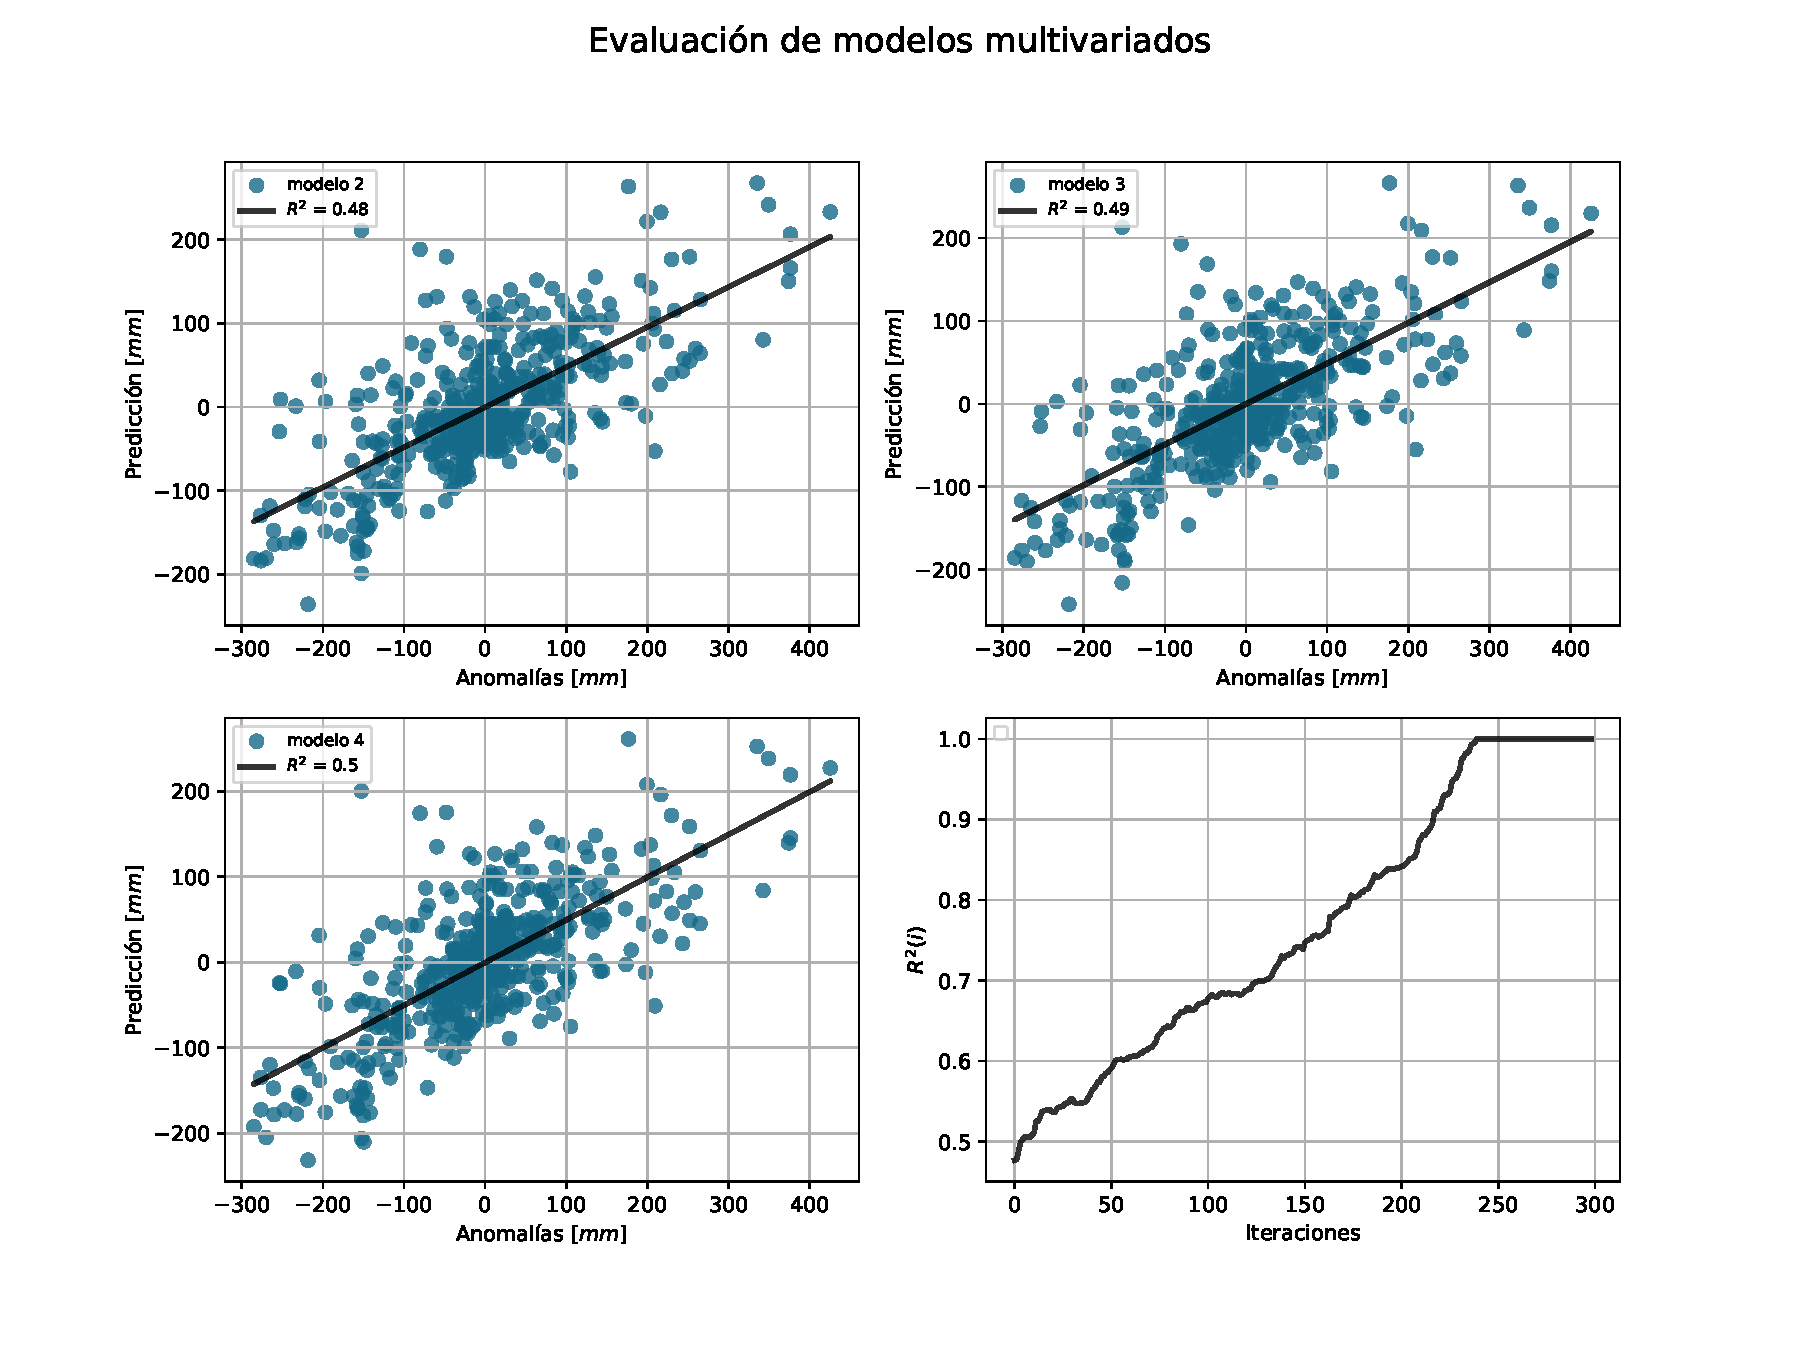
\includegraphics[width=1\textwidth]{img/model234.pdf}
\caption{\textbf{Evaluación de modelos multivariados.} Los tres diagramas de dispersión muestran el desempeño de cada uno de los tres modelos (\textit{modelo 2, modelo 3, modelo 4}). El gráfico inferior derecho muestra la evaluación de los primeros 300 modelos en los que se sumó una variable de desfase $i$.} 
\label{fig:9}
\end{figure}

\newpage

\section*{Parte 4. Evaluación de modelos para cada mes}

\bigskip

En esta ultima parte, se evaluó un modelo similar al \textit{modelo 4} pero esta vez para cada mes de manera independiente. Los resultados se pueden ver en la \textit{Figura 5}. Se observa que los modelos de los meses de verano tienen un menor rendimiento con respecto los de invierno y que el mejor rendimiento es el de octubre. Por otro lado, el rendimiento mejora con respecto al \textit{modelo 4} en los meses de abril, mayo, julio y octubre. Se puede concluir que aplicar el \textit{modelo 4} sería adecuado para análisis que abarquen todo el año, pero para análisis mas específicos, como solo el invierno, sería mas adecuado este tipo de modelos mas acotados. 

\bigskip

\begin{figure}[htp!]
\centering
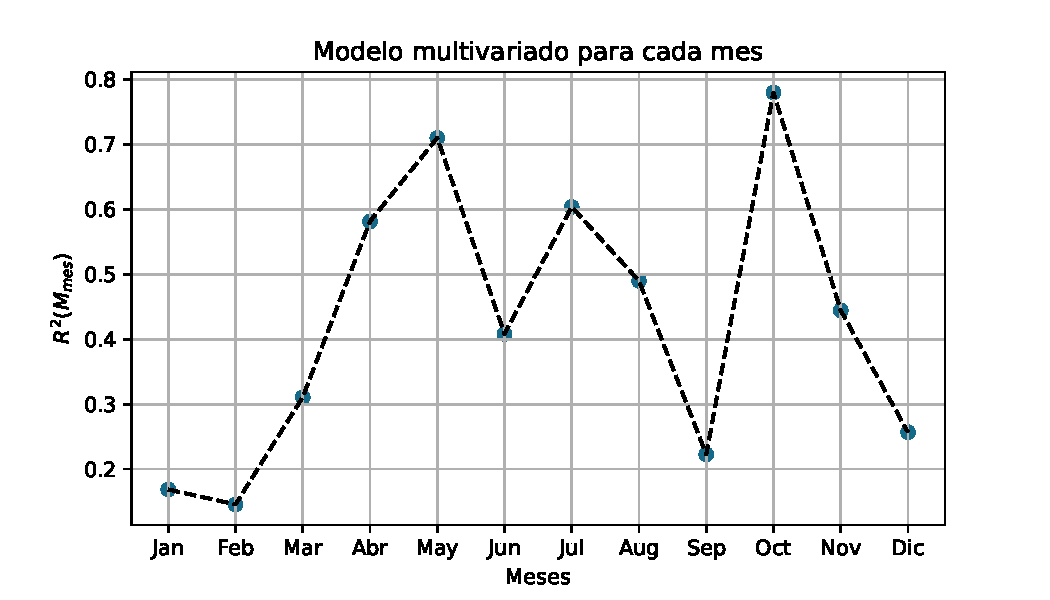
\includegraphics[width=1\textwidth]{img/modelomeses.pdf}
\caption{\textbf{Modelo multivariado para cada mes.} El gráfico muestra el desempeño de cada \textit{$modelo_{mes}$} medido en $R^{2}$.}
\label{fig:10}
\end{figure}

\newpage





% Añade una entrada a las referencias, aun cuando no esta citado explícitamente
\nocite{Wilks2006}
\nocite{Groot1992}


% Añade la bibliografía
\printbibliography
\end{document}
